\documentclass{beamer}

\usetheme{Boadilla}

\newcommand{\bi}{\begin{itemize}}
\newcommand{\ei}{\end{itemize}}
\newcommand{\be}{\begin{enumerate}}
\newcommand{\ee}{\end{enumerate}}
\newcommand{\bc}{\begin{center}}
\newcommand{\ec}{\end{center}}
\newcommand{\bd}{\begin{description}}
\newcommand{\ed}{\end{description}}
\newcommand{\I}{\item}
\newcommand{\f}{\frame}
\newcommand{\ft}{\frametitle}

\title{Offline Software Overview}
\subtitle{GlueX Collaboration Meeting}
\author[Mark Ito]{Mark M.\ Ito}
\date{February 19, 2016}
\institute[JLab]{Jefferson Lab}

\begin{document}

\f{\titlepage}

\f{\ft{Simulations for Spring 2016 Data}
  \bi
  \I Recent software changes incorporated
  \I Production has started
  \I Using SWIF-based system
  \ei
}

\f{\ft{Auto-Build and Test on Pull Request}
  \bi
  \I Sean introduced idea, MMI helped with JLab-side build scripts, Nathan added reconstruction
  \I new pull requests exist on a branch
  \I branches are checked out, compiled, and linked, log files searched for errors
  \I if build succeeds, a reconstruction test is run on small data file (real data), success evaluated
  \I result reported as comment to pull request page
  \ei
}

\f{\ft{Run Numbers: jump to the next round number}
  \bi
  \I Sean raised the issue, Justin gave example he had seen
  \I current run started with run 10,000; Fall run will start with run 20,000
  \I allows prediction of future run ranges; useful for simulation
  \I provides rough identification of run period via run number
  \ei
}

\f{\ft{Geant4}
  \bi
  \I David has demonstrated scaling of multi-threaded execution with out-of-the-box G4 version. (CPPsim)
  \I Work on hit generation continues (HDGeant4)
  \ei
}

\f{\ft{C++ Code Analyzer}
\bi
\I based on Clang/LLVM
\I reports questionable passages of code
\ei
}

\f{\ft{C++ Code Analyzer}
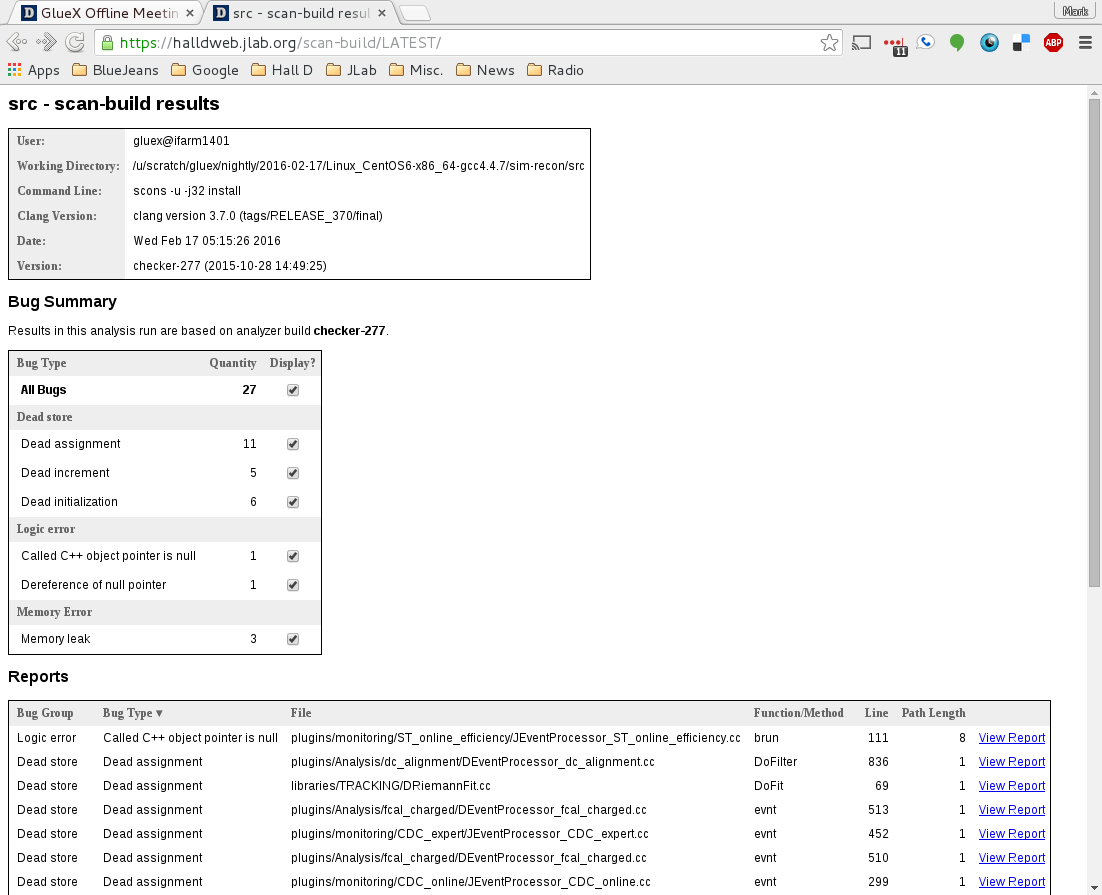
\includegraphics[width=4.5in]{code_analyzer_1.png}
}

\f{\ft{C++ Code Analyzer}
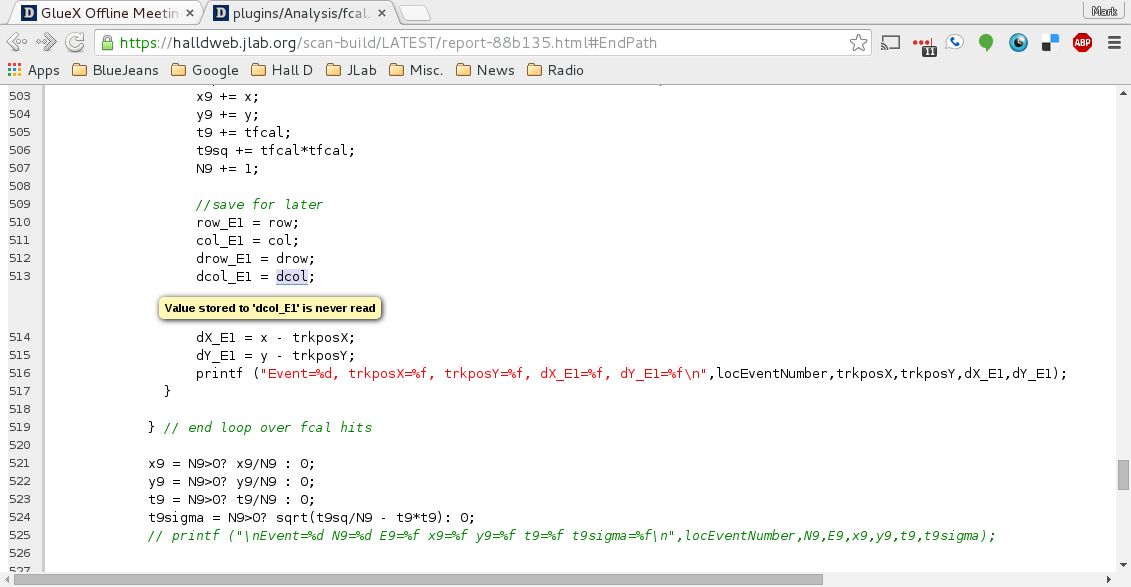
\includegraphics[width=4.5in]{code_analyzer_2.png}
}

\f{\ft{Compiler Upgrade}
}

\f{\ft{Odds and Ends}
  \bi
  \I New releases
    \bi
    \I sim-recon 1.6.0, 1.7.0
    \I HDDS 3.4, 3.5
    \I JANA 0.7.4p2
    \I CCDB 1.06.01
    \ei
  \I New Lustre-based work disk: /work/halld
  \I New Traditional work disk: /work/halld2
  \I New Private Wiki
  \I New ``Dumb offline question'' hypernews forum
  \ei
}

\f{\ft{Summary}
  \bi
  \I point 1
  \I point 2
  \ei
}

\end{document}
